\documentclass[tikz,border=5pt]{standalone}
\usepackage{amsmath,amssymb,bm}
\usetikzlibrary{arrows.meta,positioning,calc}

\definecolor{inputblue}{RGB}{222,235,247}
\definecolor{encoderblue}{RGB}{218,232,252}
\definecolor{timeblue}{RGB}{198,219,239}
\definecolor{freqgreen}{RGB}{218,240,226}
\definecolor{regionorange}{RGB}{253,228,206}
\definecolor{poolpurple}{RGB}{235,224,246}
\definecolor{headyellow}{RGB}{255,244,204}
\definecolor{ink}{RGB}{35,45,55}

\tikzset{
	flow/.style={-{Latex[length=2.4mm,width=1.6mm]},line width=0.8pt,draw=ink},
	block/.style={draw=ink,line width=0.7pt,rounded corners=3pt,align=center,
		minimum height=2.45cm,inner sep=5pt,text=ink},
	axis/.style={draw=ink!75,line width=0.6pt,rounded corners=2pt,align=center,
		minimum width=1.95cm,minimum height=3.05cm,inner sep=3pt,text=ink},
	matrixglyph/.style={draw=ink!75,line width=0.55pt,rounded corners=1pt},
	note/.style={align=center,text=ink,font=\scriptsize},
}

\begin{document}
	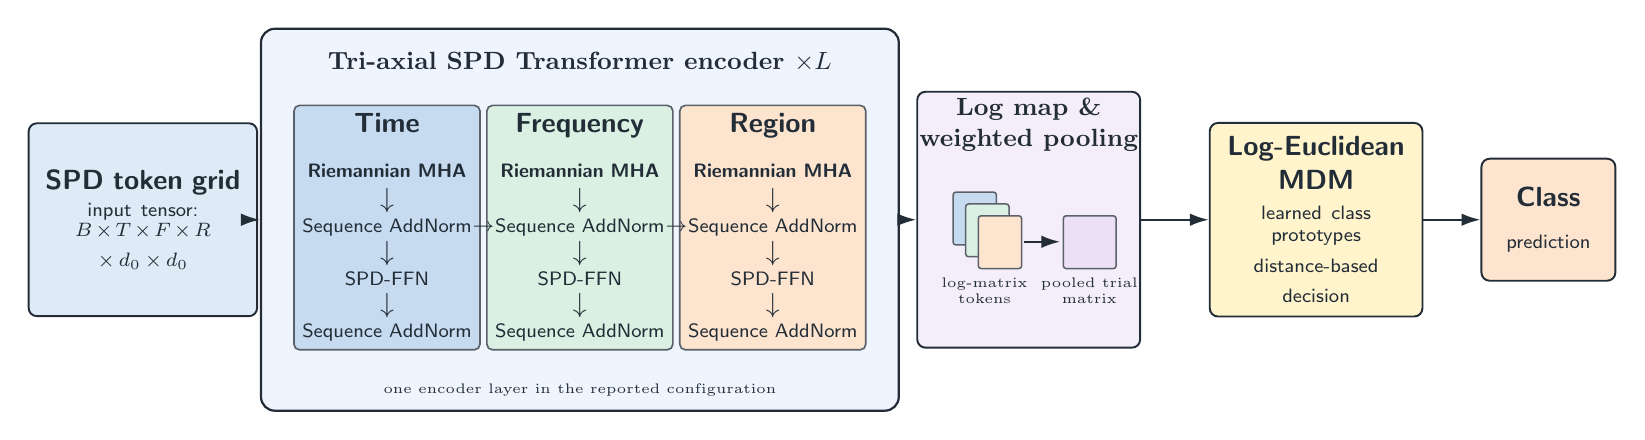
\begin{tikzpicture}[font=\sffamily]
		\node[block,fill=inputblue,text width=2.55cm] (input) at (0,0) {%
			\textbf{SPD token grid}\\[2pt]
			\scriptsize input tensor:\\[-1pt]
			$B\!\times\!T\!\times\!F\!\times\!R$\\[-1pt]
			$\times\,d_0\!\times\!d_0$
		};
		
		\node[draw=ink,line width=0.8pt,rounded corners=5pt,fill=encoderblue!42,
		minimum width=8.10cm,minimum height=4.85cm] (encoder) at (5.55,0) {};
		\node[align=center,text=ink,font=\small\bfseries] at ($(encoder.north)+(0,-0.44)$)
		{Tri-axial SPD Transformer encoder $\times L$};
		
		\node[axis,fill=timeblue] (time) at (3.10,-0.10) {%
			\textbf{Time}\\[4pt]
			\scriptsize\textbf{Riemannian MHA}\\[-1pt]
			$\downarrow$\\[-3pt]
			\scriptsize Sequence AddNorm\\[-2pt]
			$\downarrow$\\[-3pt]
			\scriptsize SPD-FFN\\[-2pt]
			$\downarrow$\\[-3pt]
			\scriptsize Sequence AddNorm
		};
		\node[axis,fill=freqgreen] (freq) at (5.55,-0.10) {%
			\textbf{Frequency}\\[4pt]
			\scriptsize\textbf{Riemannian MHA}\\[-1pt]
			$\downarrow$\\[-3pt]
			\scriptsize Sequence AddNorm\\[-2pt]
			$\downarrow$\\[-3pt]
			\scriptsize SPD-FFN\\[-2pt]
			$\downarrow$\\[-3pt]
			\scriptsize Sequence AddNorm
		};
		\node[axis,fill=regionorange] (region) at (8.00,-0.10) {%
			\textbf{Region}\\[4pt]
			\scriptsize\textbf{Riemannian MHA}\\[-1pt]
			$\downarrow$\\[-3pt]
			\scriptsize Sequence AddNorm\\[-2pt]
			$\downarrow$\\[-3pt]
			\scriptsize SPD-FFN\\[-2pt]
			$\downarrow$\\[-3pt]
			\scriptsize Sequence AddNorm
		};
		\node[font=\scriptsize,text=ink] at ($(time.east)!0.5!(freq.west)$)
		{$\rightarrow$};
		\node[font=\scriptsize,text=ink] at ($(freq.east)!0.5!(region.west)$)
		{$\rightarrow$};
		
		\node[align=center,text=ink,font=\tiny] at ($(encoder.south)+(0,0.28)$)
		{one encoder layer in the reported configuration};
		
		\node[block,fill=poolpurple!55,text width=2.48cm,minimum height=3.25cm]
		(pool) at (11.25,0) {};
		\node[align=center,text=ink,font=\small\bfseries]
		at ($(pool.north)+(0,-0.43)$) {Log map \&\\weighted pooling};
		
		% Overlapping coloured tiles denote the time/frequency/region log-matrices.
		\draw[matrixglyph,fill=timeblue]
		($(pool.center)+(-0.96,0.35)$) rectangle ++(0.55,-0.67);
		\draw[matrixglyph,fill=freqgreen]
		($(pool.center)+(-0.80,0.20)$) rectangle ++(0.55,-0.67);
		\draw[matrixglyph,fill=regionorange]
		($(pool.center)+(-0.64,0.05)$) rectangle ++(0.55,-0.67);
		\draw[flow]
		($(pool.center)+(-0.06,-0.28)$) -- ($(pool.center)+(0.40,-0.28)$);
		\draw[matrixglyph,fill=poolpurple]
		($(pool.center)+(0.44,0.05)$) rectangle ++(0.67,-0.67);
		\node[font=\tiny,text=ink,align=center]
		at ($(pool.center)+(-0.56,-0.90)$) {log-matrix\\tokens};
		\node[font=\tiny,text=ink,align=center]
		at ($(pool.center)+(0.77,-0.90)$) {pooled trial\\matrix};
		
		\node[block,fill=headyellow,text width=2.35cm] (mdm) at (14.90,0) {%
			\textbf{Log-Euclidean MDM}\\[3pt]
			\scriptsize learned class prototypes\\[3pt]
			\scriptsize distance-based\\[-1pt]
			\scriptsize decision
		};
		
		\node[block,fill=regionorange,text width=1.35cm,minimum height=1.55cm]
		(output) at (17.85,0) {\textbf{Class}\\[3pt]\scriptsize prediction};
		
		\draw[flow] (input.east) -- (encoder.west);
		\draw[flow] (encoder.east) -- (pool.west);
		\draw[flow] (pool.east) -- (mdm.west);
		\draw[flow] (mdm.east) -- (output.west);
		
	\end{tikzpicture}
\end{document}
